\section{Results}
\label{results}

We compared the performance of the proposed methods by estimating the two structural 
parameters of interest $\tau_F$ and $\tau_C$ using the weighted least squares. 
For FE-MSM, the parameters are estimated by solving the following optimization problem:
\begin{equation}
\label{eq:least_squares}
(\widehat{\tau}_F,\widehat{\tau}_C)
=
\arg\min_{\tau_F',\tau_C'}
\sum_{i=1}^{n}
\widehat{W}_i
\left\{
Y_i-\alpha-\tau_F' A_{iT}
-\tau_C' \sum_{t=T-1}^{T-3} A_{it}
\right\}^{2}
\end{equation}
Where $\widehat{W}_i$ are the stabilized version of 
IPTW weights defined in Eq.~\eqref{eq:iptw_weights}. 
The parametric 
propensity score model is correctly specified (up to a unit-specific fixed effect) 
as a logistic regression of the 
treatment on the past treatment history and covariates, with a unit-specific fixed effect, 
\begin{equation}
\label{eq:ps_model}
p(a_{it} = 1 \mid x_{it}, a_{i,t-1}, z_i^{(s)}) = \operatorname{expit}(w_1^\top x_{it} + w_2 a_{i,t-1} + \alpha_i).
\end{equation}


For the sequential GPLVM, a $\text{CMM}(1)$ with a one dimensional latent variable 
(i.e., $Z_i \in \mathbb{R}$ and $|\mathcal{Z}| = 1$) 
is fitted to the treatment data, 
using a linear kernel: 
\[
k_t^{\text{treat}} ((x_t,a_{t-1},z), (x'_t,a'_{t-1},z'))= \nu \left[\sum_{j=1}^{|\mathcal{X_t}|}x_{jt} x'_{jt} 
+ aa' + \sum_{j=1}^{|\mathcal{Z}|} z_{j} z'_{j} \right]
\]
where $\nu$ is the variance hyperparameter. This is equivalent to 
the Bayesian linear regression with a latent variable. The observed confounders 
are standardized before fitting the GPLVM. A  
weakly informative Gamma prior is placed on 
$\nu$, specifically $\nu \sim \Gamma(2,1)$.
The parameters of the GPLVM are estimated by minimizing the negative evidence 
lower bound using the Adam optimizer with learning rate set to 
$0.01$. The number of iterations is set to $6000$ and the convergence is 
monitored by checking the change in ELBO.
The parameters of the MSM are estimated by
the procedure described in Section~\ref{sec:seqgplvm-outcome} by solving 
the same optimization problem as in Eq.~\eqref{eq:least_squares} with 
number of posterior draws set to $S=100$. The following logistic regression 
model is used to estimate the propensity scores for the IPTW estimation 
of the MSM parameters:
\begin{equation}
\label{eq:ps_model_seqgplvm}
p(a_{it} = 1 \mid x_{it}, a_{i,t-1}, z_i^{(s)}) = 
\operatorname{expit}\!\left(w_3^\top x_{it} + w_4 a_{i,t-1}+ w_5 z_i^{(s)}+ w_6 \right),
\end{equation}
where $z_i^{(s)}$ is the $s$-th posterior draw of the latent variable for individual $i$.

For both methods, the weighting is stabilized by multiplying the weights with 
conditional probabilities of the current treatment given only the previous treatment using 
the following logistic regression model:
\begin{equation}
\label{eq:ps_model_stabilized}
p(a_{it} = 1 \mid a_{i,t-1}) = \operatorname{expit}\!\left(w_7 a_{i,t-1} + w_8\right).
\end{equation}


\paragraph{Treaming weights.} The unit-specific fixed effects and the individual latent variables are not identified 
for individuals with no variation in their treatment history, i.e., always 
treated or never treated. Including these samples in the estimation process can make the optimizations 
for both methods unstable. Even if the population level positivity assumption holds, 
in the finite sample, it is 
possible to have such individuals. This problem becomes more severe when the number of time points is small. 
In this case, we removed always/never treated 
individuals from the estimation process and imputed their propensity 
scores by assigning a fixed value, e.g., $\hat{\pi}_{it} = 0.01$ for never treated 
individuals and $\hat{\pi}_{it} = 0.99$ for always treated individuals for all 
time points. Depending on the lenght of the treatment intervention window $k$ specified 
in the MSM, this imputation strategy can lead to extream weights which 
we further treamed by capping them within the range of $[10^{-6}, 1-10^{-6}]$ 
to avoid unstable weights. 

Figure~\ref{fig:simulation_results} shows the results of the simulation study for the 
two covariate case. Bias, standard deviation, and coverage of the 
95\% confidence intervals are reported based on 500 simulation runs. The first 
two columns correspond to the weak unmeasured confounding setting where 
$U_i \in [-1,1]$ and 
the last two columns correspond to the strong unmeasured confounding 
setting where $U_i \in [-2,2]$. Solid lines in grey show the results using the 
true propensity scores (\texttt{IPTW-True}). Solid orange lines 
show the results for FE-MSM (\texttt{IPTW-FE-impute}) and dashed 
purple lines show the results for SeqGPLVM (\texttt{IPTW-SeqGPLVM-impute}). 
Dashed blue lines 
represent the results for the naive IPTW estimaton of the specified MSM assuming 
sequential ignorability without adjusting for the unmeasured confounder (\texttt{IPTW}). 
In this case we used the same logistic regression as 
in Eq.~\eqref{eq:ps_model} to estimate the propensity scores by replacing 
the individual 
fixed effects $\alpha_i$ with a global intercept. Shapes 
correspond to the $n$ to $T$ ratio. Squares represent $\rho = 5$ (the largest number of time points), 
circles represent $\rho = 10$, and triangles represent $\rho = 50$ (the smallest number of time points). 

The results show that both methods improves the bias of the estimates of the 
parameters of interest in comparison to the naive IPTW, especially as the ratio of 
$\frac{n}{T}$ increases. However, the FE-MSM method tends to have slightly lower bias and 
standard error compared to the sequential GPLVM method, particularly for smaller sample sizes. 
This may be due to the fact that the FE-MSM method relies on a correctly specified 
parametric model for the propensity scores, while the sequential GPLVM method is more 
flexible but may require larger sample sizes to achieve similar performance. We can see that 
the worst case for both methods is for $\rho = 50$ but specially this is visible for 
the sequential GPLVM in the smallest sample size $N = 200$, Where it introduces 
more bias than the naive IPTW for the strong unmeasured confounding case ($a = 2$) 
and performs almost equally as the naive IPTW for the weak unmeasured confounding 
case ($a = 1$). However, 
since the standard error of the estimates is also larger in this case, 
the coverage of the confidence intervals is still close to the nominal level. This indicates that SeqGPLVM 
can still provide a reasonable uncertainty quantification even in the worst case scenario by being 
less certain about the estimates in comparison to the naive IPTW. 

As the number of time points increases, the gap between the bias of two methods decreases and 
they perform more similarly although the FE-MSM bias remains lower while the standard 
error of SeqGPLVM the estimates remains higher than the FE-MSM estimates across all scenarios. 
Under the weak unmeasured confounding setting where the unmeasured confounder explains 
roughly 1/3 of the variance of the treatment assignments, the confidence interval 
estimates of the two methods stays close to the nominal coverage except for the shortest treatment 
sequence and $N = 500$ and $N = 1000$ where the coverage of the confidence intervals for 
the sequential GPLVM method is much lower than the nominal level. 
This is likely due to the fact that the bias of the estimates is larger than the standard error in this case which leads to undercoverage of the confidence intervals. However, for other scenarios, the coverage of the confidence intervals for both methods is close to the nominal level and FE-MSM performs almost the same as the true propensity case even for the shortest treatment sequence $t = 4$.
slightly lower than the nominal level. Under this scenario FE-MSM performs almost the same as the true propensity case even for the shortest treatment sequence $t = 4$. In the stronger unmeasured confounding case where the unmeasured confounder explains roughly 2/3 of the variance in the treatment, both methods perform more poorly than the weaker case in terms of bias while FE-MSM performs slightly better across all rhos and sample sizes. In this case there is a larger gap between the bias of two methods especially for smaller sample sizes and shorter treatment sequences. However, as the number of time points increases, this gap decreases and both methods perform more similarly although FE-MSM still has lower bias and standard error compared to SeqGPLVM across all scenarios.
in terms of bias and standard error. Under the weak unmeasured confoundedness

\begin{itemize}
    \item worst case for both method is for rho = 50 but specially this is visible for 
    seqgplvm more than femsm. in the smallest 
    individual size N = 200, performs equally as the naieve IPTW (a = 1) or even more biased (a = 2) in both case 
    with larger standard error. Hence, femsm performs 
    better with shorter time periods. This is expected since seqgplvm has much more parameters 
    and requires more data for training
    \item as the number of time points increases, the gap between the bias of two methods 
    decreases and they perform more similarly although the Fe-MSM bias remains lower in terms of bias and standard error.
    \item under the weak unmeasured confoundedness the where the unmeansured confounder explains roughly 1/3 
    of the variance of the treatment assignments, the confidence interval estimates of 
    the two methods stays close to the nominal coverage across different values of n and p. 
    Under this scenario FE-MSM performs almost the same as the true propensity case even for 
    the shortest treatment sequence t = 4. 
    \item in the stronger unmeasured confoundedness case where the unmeasured confounder explains 
    2/3 of the variance in the treatment, both methods perform more poorly 
    than the weaker case in terms of the bias while FE msm perfroms slightly better across all rhos and 
    sample sizes. in this case there 


\end{itemize}


naive model that does not adjust for the unmeasured confounder 
(\texttt{IPTW}), dashed line in light blue shows the results for the
dashed line in green shows the results for the
IPTW method using the estimated propensity scores from the correctly specified logistic regression model (\texttt{IPTW}), dashed line
in orange shows the results for the 
FE-MSM method and dashed line in purple shows the results for the 
sequential GPLVM. The first two columns correspond to the weak unmeasured confounding setting ($\rho=5$)

 and the last two columns correspond to the strong unmeasured confounding setting ($\rho=50$). The first row corresponds to the estimation of $\tau_F$ and the second row corresponds to the estimation of $\tau_C$. The results for $a=1$ and $a=2$ are shown in the left and right panels, respectively. 
The results show that both methods can estimate the parameters of interest with low bias and good coverage, especially as the number of individuals increases. However, the FE-MSM method tends to have slightly lower bias and better coverage compared to the sequential GPLVM method, particularly for smaller sample sizes. This may be due to the fact that the FE-MSM method relies on a correctly specified parametric model for the propensity scores, while the sequential GPLVM method is more flexible but may require larger sample sizes to achieve similar performance.
\begin{figure}[t]
    \centering
    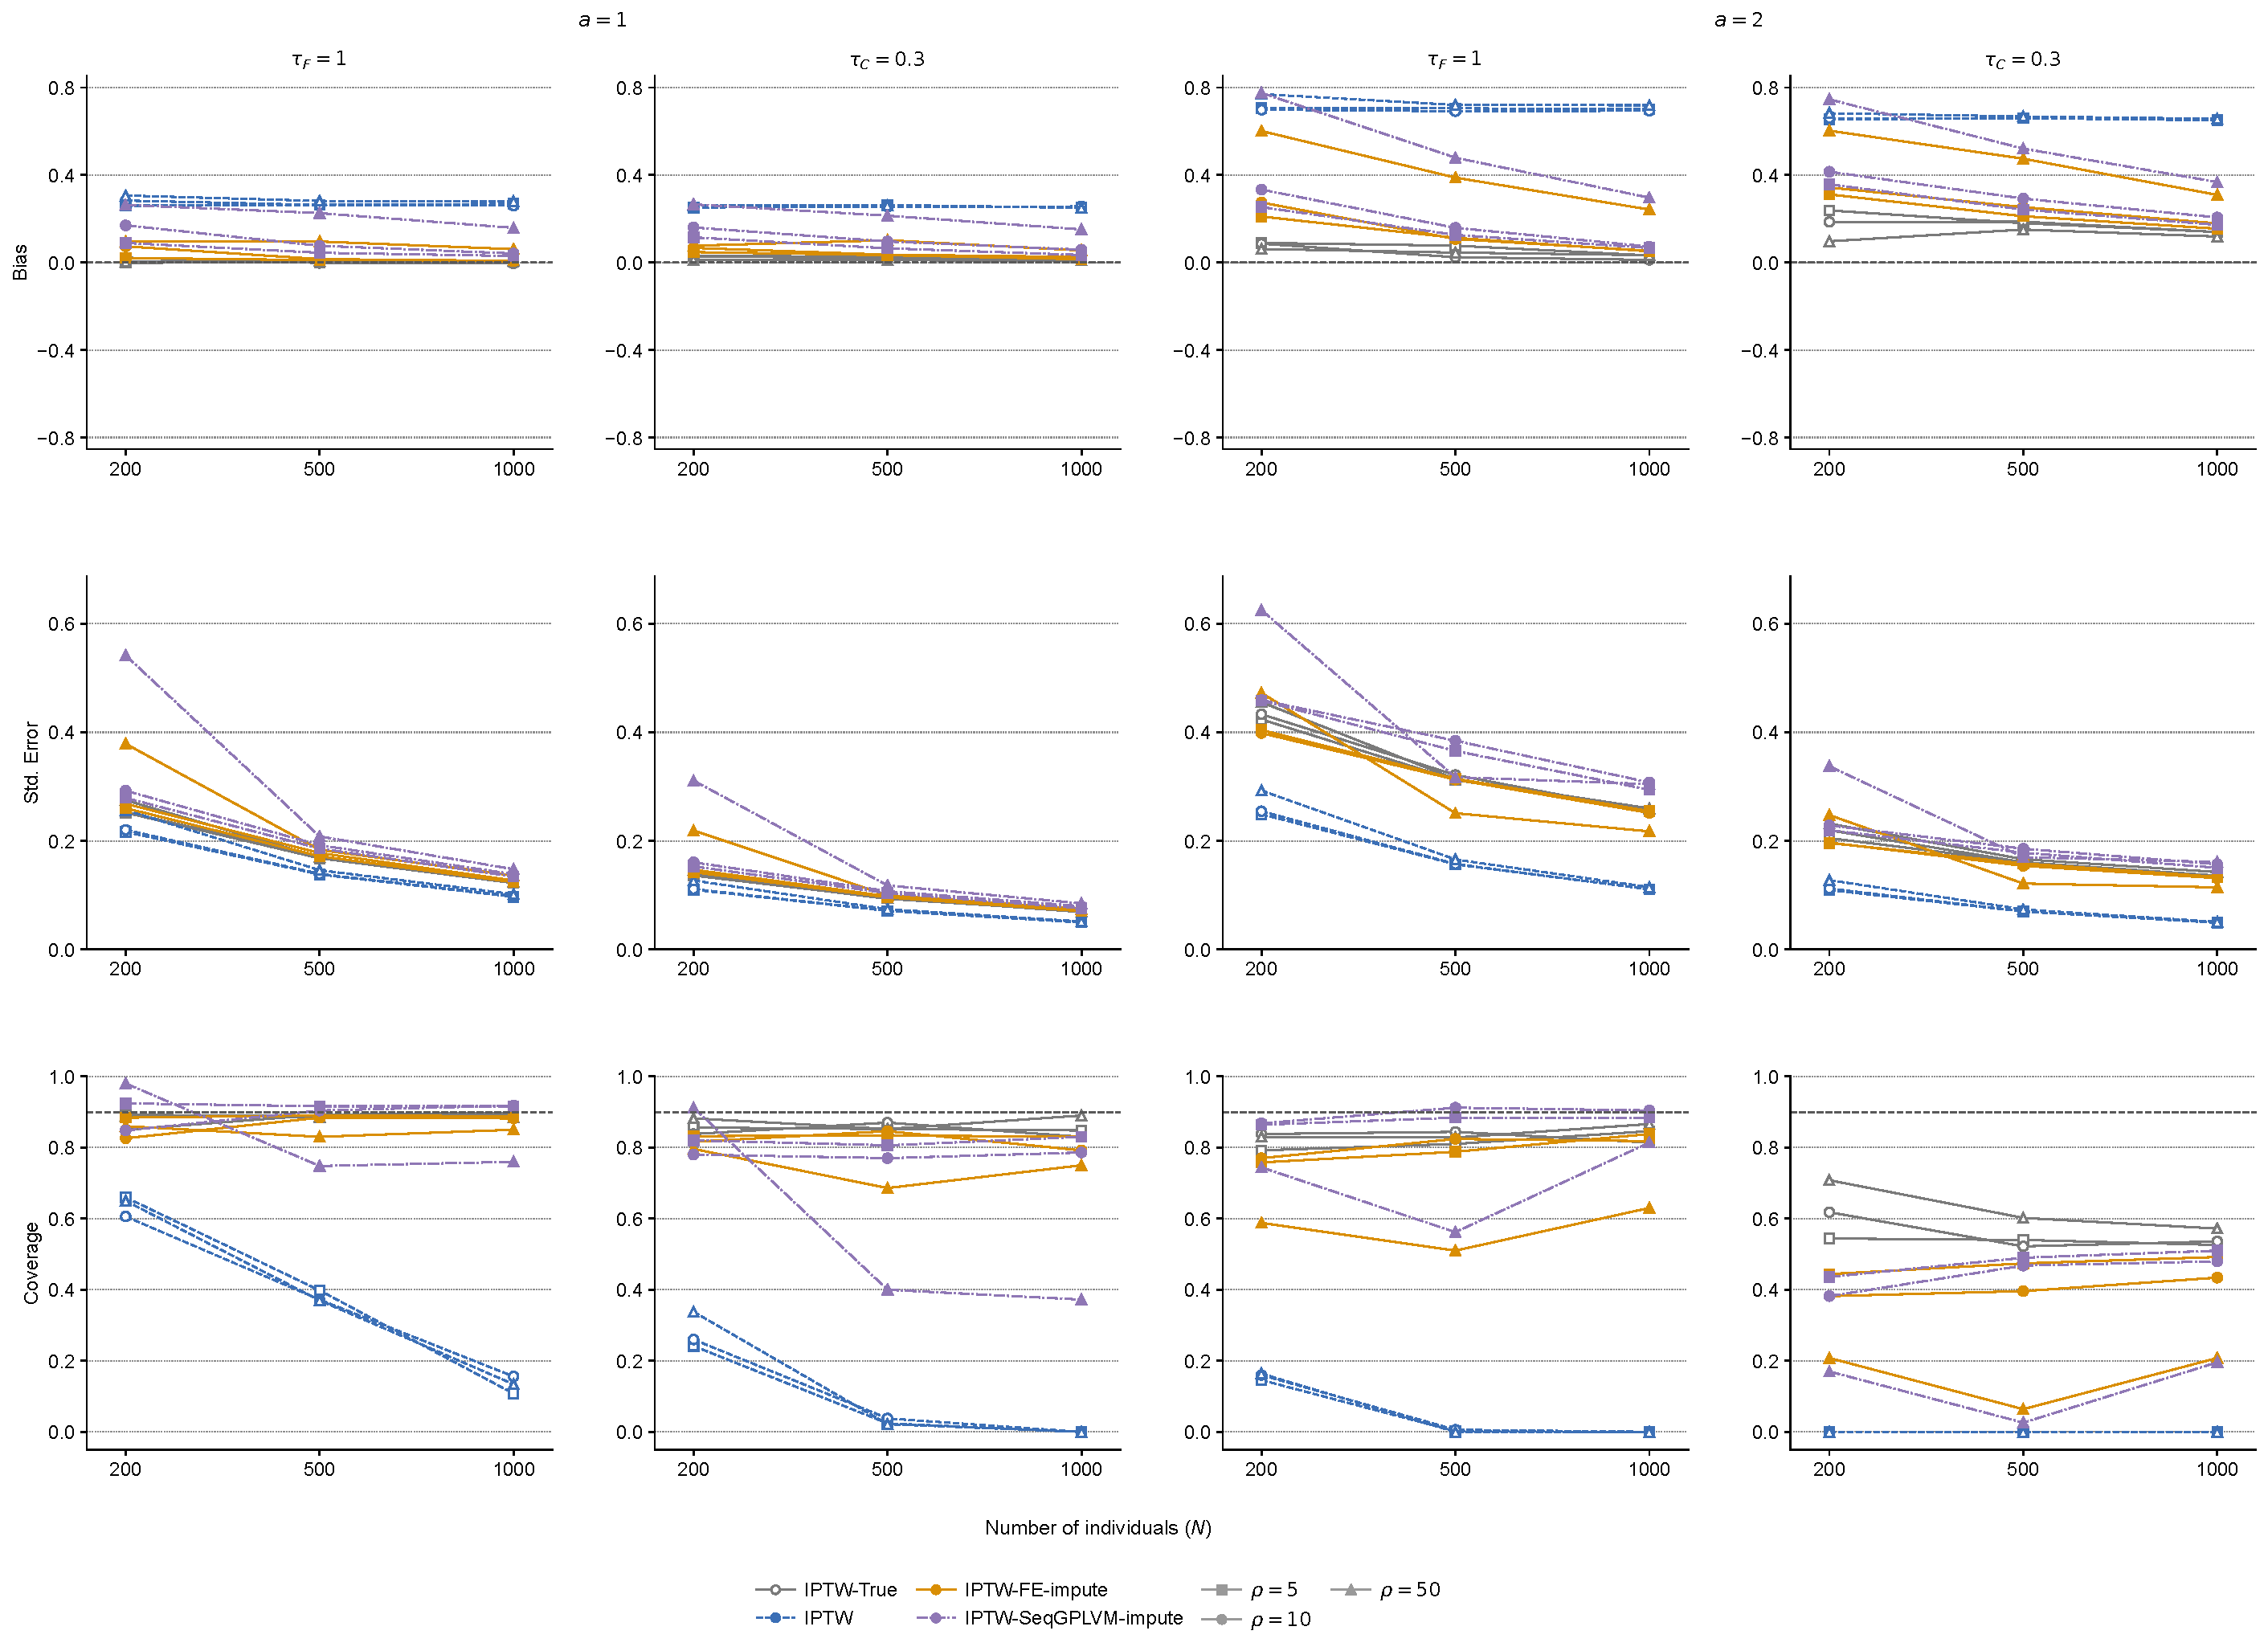
\includegraphics[width=1\textwidth]{figures/build/simulation_results.pdf}
    \caption{Simulation results for FE-MSM and sequential GPLVM.}
    \label{fig:simulation_results}
\end{figure}
\textbf{DISCUSSION}
\hl{While this MI-style propagation provides a principled empirical uncertainty summary,
it does not close the main theoretical gap in the sequential deconfounding approach.
First, it does not by itself deliver a large-sample result for the \emph{overall}
two-stage estimator---i.e., conditions under which the plug-in (or draw-averaged)
MSM estimator is consistent and $\sqrt{N}$-asymptotically normal with a valid variance
formula---of the kind established for FE--IPTW by Blackwell and Yamauchi.
Second, because the outcome stage is not modeled jointly with the treatment model,
the distribution of $\{\hat{\gamma}^{(s)}\}$ should be interpreted as uncertainty
propagation rather than a coherent Bayesian posterior for $\gamma$; consequently,
interval calibration is not automatically guaranteed from Bayesian first principles.
Third, even perfect variance combination does not address potential sources of
systematic error---such as misspecification of the latent treatment model/CMM,
violations of positivity leading to unstable weights, or approximation error from
variational inference---which can affect both bias and coverage.}